\documentclass{article}

\usepackage{arxiv}

\usepackage[utf8]{inputenc} % allow utf-8 input
\usepackage[T1]{fontenc}    % use 8-bit T1 fonts
\usepackage{lmodern}        % https://github.com/rstudio/rticles/issues/343
\usepackage{hyperref}       % hyperlinks
\usepackage{url}            % simple URL typesetting
\usepackage{booktabs}       % professional-quality tables
\usepackage{amsfonts}       % blackboard math symbols
\usepackage{nicefrac}       % compact symbols for 1/2, etc.
\usepackage{microtype}      % microtypography
\usepackage{lipsum}
\usepackage{graphicx}

\title{Spatial Scales of Local Adaptation and Host-Parasite Coevolution}

\author{
    Bob Week
   \\
    Integrative Biology \\
    Michigan State University \\
  East Lansing, MI 48824 \\
  \texttt{\href{mailto:weekrobe@msu.edu}{\nolinkurl{weekrobe@msu.edu}}} \\
   \And
    Gideon Bradburd
   \\
    Integrative Biology \\
    Michigan State University \\
  East Lansing, MI 48824 \\
  \texttt{\href{mailto:bradburd@msu.edu}{\nolinkurl{bradburd@msu.edu}}} \\
  }


% Pandoc citation processing
\newlength{\csllabelwidth}
\setlength{\csllabelwidth}{3em}
\newlength{\cslhangindent}
\setlength{\cslhangindent}{1.5em}
% for Pandoc 2.8 to 2.10.1
\newenvironment{cslreferences}%
  {}%
  {\par}
% For Pandoc 2.11+
\newenvironment{CSLReferences}[3] % #1 hanging-ident, #2 entry spacing
 {% don't indent paragraphs
  \setlength{\parindent}{0pt}
  % turn on hanging indent if param 1 is 1
  \ifodd #1 \everypar{\setlength{\hangindent}{\cslhangindent}}\ignorespaces\fi
  % set entry spacing
  \ifnum #2 > 0
  \setlength{\parskip}{#2\baselineskip}
  \fi
 }%
 {}
\usepackage{calc} % for calculating minipage widths
\newcommand{\CSLBlock}[1]{#1\hfill\break}
\newcommand{\CSLLeftMargin}[1]{\parbox[t]{\csllabelwidth}{#1}}
\newcommand{\CSLRightInline}[1]{\parbox[t]{\linewidth - \csllabelwidth}{#1}}
\newcommand{\CSLIndent}[1]{\hspace{\cslhangindent}#1}

\usepackage{amsmath}
\usepackage{mathrsfs}
\usepackage{csquotes}
\usepackage{textcomp}
\usepackage[T3,T1]{fontenc}
\DeclareSymbolFont{tipa}{T3}{cmr}{m}{n}
\DeclareMathAccent{\invbreve}{\mathalpha}{tipa}{16}


\begin{document}
\maketitle

\def\tightlist{}


\begin{abstract}
Studies of local adaptation between coevolving hosts and parasites have
profited from theory that assumes a discrete set of populations.
However, when dispersal is limited clinal patterns of phenotypic
variation may emerge. Thus, patterns of local adaptation may occur on
characteristic spatial scales determined by dispersal distances and
strengths of coevolutionary selection. Here we study a two-dimensional
continuous space model of host-parasite coevolution to understand the
relative spatial scales of phenotypic turnover and local adaptation. We
find that the species with more limited dispersal tends to be locally
adapted, but XYZ about it being ahead in the coevolutionary race. To
verify our results when model assumptions are broken, we use individual
based simulations. We find XYZ about our results when coevolution is
strong and XYZ when population densities significantly vary across
space.
\end{abstract}

\keywords{
    coevolution
   \and
    local adaptation
   \and
    continuous space
   \and
    characteristic scales
   \and
    spde
  }

\hypertarget{introduction}{%
\section{Introduction}\label{introduction}}

\begin{itemize}
\item
  It seems an old motivation for studying local adaptation in
  host-parasite coevolution comes from trying to make sense of the GMTC.
  So I think it would be good to include this.
\item
  Need to do lit review of local adaptation in coevolving host-parasite
  systems.
\item
  We should also tie in previous work on understand spatial scales of
  phenotypic variation (ie, Slatkin's 1978 ppr). Need to do lit review
  in this area too.
\end{itemize}

\hypertarget{methods}{%
\section{Methods}\label{methods}}

\hypertarget{spde-model}{%
\subsection{SPDE Model}\label{spde-model}}

\ldots{}

The assumption of constant effective population size across time and
space can be thought of as an extreme form of population regulation.
However, the model is agnostic to whether population regulation is
caused by top-down forces such as predation, bottom-up forces such as
resource competition or some combination of these forces.

\hypertarget{individual-based-simulations}{%
\subsection{Individual-Based
Simulations}\label{individual-based-simulations}}

\hypertarget{results}{%
\section{Results}\label{results}}

\hypertarget{discussion}{%
\section{Discussion}\label{discussion}}

\hypertarget{conclusion}{%
\section{Conclusion}\label{conclusion}}

\newpage

\appendix

\begin{center}
\Large{Appendix}
\end{center}

\hypertarget{calculating-the-covariance-and-cross-covariance-functions}{%
\section{Calculating the covariance and cross-covariance
functions}\label{calculating-the-covariance-and-cross-covariance-functions}}

To compute formula for the spatial (intraspecific) covariance and
(interspecific) cross-covariance functions, we make use of the relation
between the covariance functions and power spectra of random fields. In
particular, the power spectrum of a multivariate stationary random field
\(\pmb F(\pmb x)\), \(\pmb x=(x_1,x_2)\) being spatial location, is
defined by
\(S_{\pmb F}(\pmb k)=\mathbb E\left(\hat{\pmb F}(\pmb k)\hat{\pmb F}(\pmb k)^H\right)\)
where \(\hat{\pmb F}(\pmb k)\) is the Fourier transform of \(\pmb F\),
the symbol \(^H\) denotes Hessian transpose and \(\pmb k=(k_1,k_2)\) are
the Fourier transformed coordinates which represent the frequencies of
fluctuations across the two spatial dimensions. Hence, \(\hat{\pmb F}\)
represents the harmonic content of the process \(\pmb F\). The spatial
covariance function \(C_{\pmb F}(\pmb x)\) is just the inverse Fourier
transform of the power spectrum \(S_{\pmb F}(\pmb k)\).

Working with the power spectrum has the advantage of converting
differential equations into algebraic equations, making for a more
analytically tractable approach. Furthermore, due to the Fourier
relationship between \(C_{\pmb F}(\pmb x)\) and \(S_{\pmb F}(\pmb k)\),
we have the convenient properties
\(\int_{\mathbb R^2}C_{\pmb F}(\pmb x)d\pmb x=S_{\pmb F}(\pmb 0)\) and
\(\int_{\mathbb R^2}S_{\pmb F}(\pmb x)d\pmb x=C_{\pmb F}(\pmb 0)\). Both
of these properties will aid in calculating results on host-parasite
local adaptation.

Using \(\pmb k=(k_1,k_2)\) to denote spatial frequency (the Fourier
equivalent to spatial location \(\pmb x=(x_1,x_2)\)) and
\(\hat{\pmb z}(\pmb k)=(\hat z_H(\pmb k),\hat z_P(\pmb k))^\top\) to
denote the Fourier transforms of the equilibrium solution
\(\bar{\pmb z}(\pmb x)=(\bar z_H(\pmb x),\bar z_P(\pmb x))^\top\), the
Fourier transform of our model at equilibrium is

\[0=G_HA_H(\theta_H-\hat z_H)-G_HB_H(\hat z_P-\hat z_H)-\frac{\sigma_H^2}{2}\|\pmb k\|^2\hat z_H+\sqrt\frac{G_H}{N_H}\widehat{\dot W}_H,\]

\[0=G_PA_P(\theta_P-\hat z_P)+G_PB_P(\hat z_H-\hat z_P)-\frac{\sigma_P^2}{2}\|\pmb k\|^2\hat z_P+\sqrt\frac{G_P}{N_P}\widehat{\dot W}_P,\]

where \(\|\pmb k\|^2=k_1^2+k_2^2\) and \(\widehat{\dot W}_S\) is a
heuristic representation for the Fourier transform of the spatial white
noise \(\dot W_S\) for species \(S=H,P\). Since the mean vector for
equilibrium solution of the SPDE model is spatially homogeneous, we set
\(\theta_H=\theta_P=0\) without loss of generality. This is equivalent
to centering the solution by working with \(\tilde z_H=\bar z_H-\mu_H\)
and \(\tilde z_P=\bar z_P-\mu_P\) instead of \(\bar z_H\) and
\(\bar z_P\). The Fourier transformed SPDE model can be rewritten in
matrix form as

\[\mathscr H\hat{\pmb z}=\widehat{\dot{\pmb W}}\]

where
\(\widehat{\dot{\pmb W}}=\tfrac{1}{2\pi}\left(-\sqrt{\tfrac{G_H}{N_H}}\hat{\dot W}_H, -\sqrt{\tfrac{G_P}{N_P}}\hat{\dot W}_P\right)^\top\)
and

\[\mathscr H=\frac{1}{2\pi}\left(\begin{matrix}-G_HA_H+G_HB_H+\frac{\sigma_H^2}{2}\|\pmb k\|^2 & -G_HB_H \\ G_PB_P & -G_PA_P-G_PB_P+\frac{\sigma_P^2}{2}\|\pmb k\|^2\end{matrix}\right).\]

Since no complex numbers appear in the above expressions, the power
spectrum of the random field \(\bar{\pmb z}\) simplifies to
\(S_{\bar{\pmb z}}=\mathbb E\left(\hat{\pmb z}\hat{\pmb z}^\top\right)\).
Rearranging the above matrix equation, we find

\[\hat{\pmb z}=\mathscr H^{-1}\widehat{\dot{\pmb W}},\]

\[\hat{\pmb z}^\top=\widehat{\dot{\pmb W}}^\top\left(\mathscr H^\top\right)^{-1}.\]

Hence, the power spectrum of \(\bar{\pmb z}\) is

\[S_{\bar{\pmb z}}=\mathscr H^{-1}S_{\dot{\pmb W}}\left(\mathscr H^\top\right)^{-1}\]

where

\[S_{\dot{\pmb W}}=\mathbb E\left(\widehat{\dot{\pmb W}}\widehat{\dot{\pmb W}}^\top\right)=\frac{1}{(2\pi)^2}\left(\begin{matrix}G_H/N_H & 0 \\ 0 & G_P/N_P \end{matrix}\right)\]

is the power spectrum of the spatial white noise
\(\dot{\pmb W}=\left(-\sqrt{\tfrac{G_H}{N_H}}{\dot W}_H, -\sqrt{\tfrac{G_P}{N_P}}{\dot W}_P\right)^\top\).
Denoting \(S_H,S_P\) and \(S_{HP}\) the components of
\(S_{\bar{\pmb z}}\) corresponding to the host power spectrum, parasite
power spectrum and host-parasite cross-power spectrum we find

\[S_H(\pmb k)=\frac{B_H^2G_H^2\frac{G_P}{N_P}+\frac{G_H}{N_H}\big[G_P(A_P+B_P)+\frac{1}{2}\sigma_P^2\|\pmb k\|^2\big]^2}{\big\{B_HB_PG_HG_P+[G_H(A_H-B_H)+\frac{1}{2}\sigma_H^2\|\pmb k\|^2][G_P(A_P+B_P)+\frac{1}{2}\sigma_P^2\|\pmb k\|^2]\big\}^2},\]

\[S_P(\pmb k)=\frac{B_P^2G_P^2\frac{G_H}{N_H}+\frac{G_P}{N_P}\big[G_H(A_H-B_H)+\frac{1}{2}\sigma_H^2\|\pmb k\|^2\big]^2}{\big\{B_HB_PG_HG_P+[G_H(A_H-B_H)+\frac{1}{2}\sigma_H^2\|\pmb k\|^2][G_P(A_P+B_P)+\frac{1}{2}\sigma_P^2\|\pmb k\|^2]\big\}^2},\]

\[S_{HP}(\pmb k)=\frac{B_PG_P\frac{G_H}{N_H}\big[G_P(A_P+B_P)+\frac{1}{2}\sigma_P^2\|\pmb k\|^2\big]-B_HG_H\frac{G_P}{N_P}\big[G_H(A_H-B_H)+\frac{1}{2}\sigma_H^2\|\pmb k\|^2\big]}{\big\{B_HB_PG_HG_P+[G_H(A_H-B_H)+\frac{1}{2}\sigma_H^2\|\pmb k\|^2][G_P(A_P+B_P)+\frac{1}{2}\sigma_P^2\|\pmb k\|^2]\big\}^2}.\]

Assuming coevolution is weak so that \(B_H^2,B_P^2,B_HB_P\approx0\), we
obtain the approximations

\[S_H(\pmb k)\approx\frac{G_H/N_H}{\left(G_H(A_H-B_H)+\frac{\sigma_H^2}{2}\|\pmb k\|^2\right)^2}, \ S_P(\pmb k)\approx\frac{G_P/N_P}{\left(G_P(A_P+B_P)+\frac{\sigma_P^2}{2}\|\pmb k\|^2\right)^2}\]

\[S_{HP}(\pmb k)\approx\frac{B_PG_HG_P/N_H}{\left(G_H(A_H-B_H)+\frac{\sigma_H^2}{2}\|\pmb k\|^2\right)^2\left(G_P(A_P+B_P)+\frac{\sigma_P^2}{2}\|\pmb k\|^2\right)}\]

\[-\frac{B_HG_HG_P/N_P}{\left(G_H(A_H-B_H)+\frac{\sigma_H^2}{2}\|\pmb k\|^2\right)\left(G_P(A_P+B_P)+\frac{\sigma_P^2}{2}\|\pmb k\|^2\right)^2}.\]

In Figure 1, we compare these approximations to the exact power spectra
for varying strengths of coevolutionary selection.

\begin{figure}
\centering
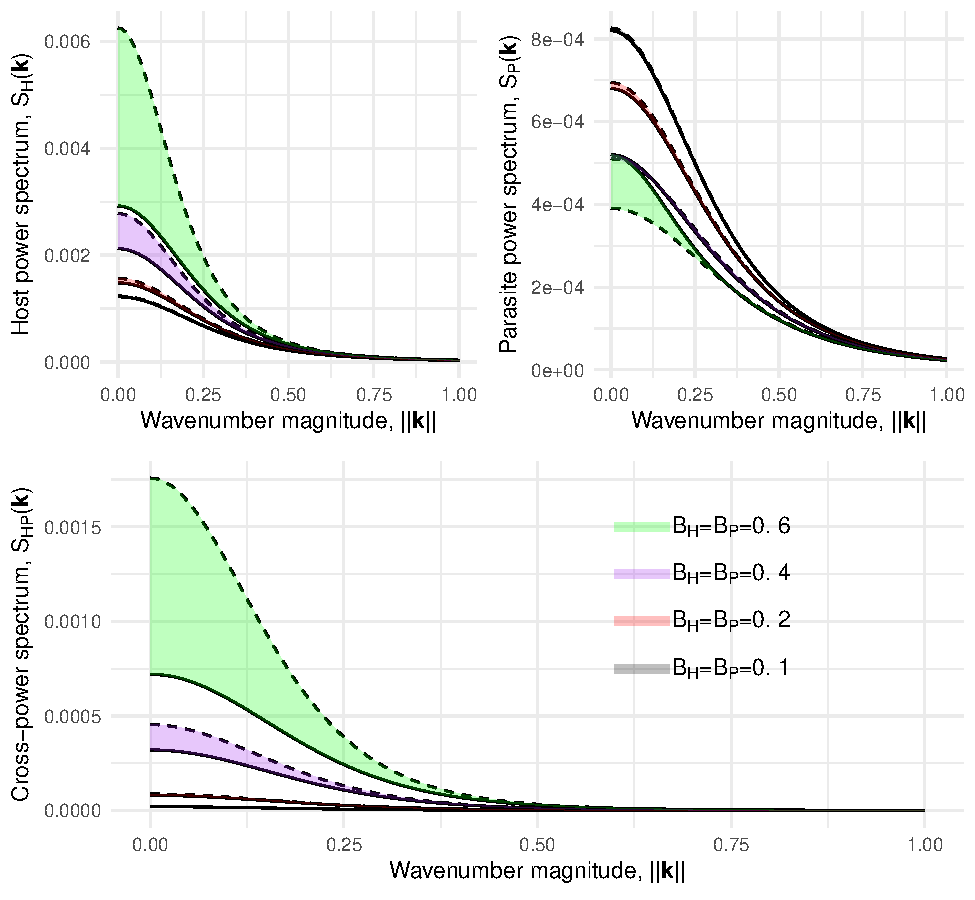
\includegraphics{Spatial-Scales-of-Local-Adaptation-in-Host-Parasite-Coevolution_files/figure-latex/unnamed-chunk-1-1.pdf}
\caption{Comparisons of approximated power spectra (dashed lines) to
exact power spectra (solid lines) for four different strengths of biotic
(coevolutionary) selection \(B=0.1,0.2,0.4,0.6\). For simplicity, biotic
selection on host and parasite are set equal (\(B_H=B_P=B\)). Background
parameters are set to \(A_H=A_P=1\), \(G_H=G_P=10\),
\(\sigma_H=\sigma_P=10\) and \(N_H=N_P=100\). Our model only is defined
for \(B_H<A_H\). Hence, the behaviour of power spectra as \(B\)
increases reflects what happens when the host comes closer to being able
to overcome abiotic stabilizing selection and escape parasitism. In this
limit, we see that our approximations over estimate the magnitudes of
low frequency content in the host spatial covariance and host-parasite
cross-covariance. This implies that our approximations over estimate the
spatial scale of phenotypic covariance of the host and phenotypic
cross-covariance of the host and parasite when coevolution is strong. In
contrast, we see that our approximations under estimate the amount of
low frequency content in the spatial covariance of parasite traits. This
implies that our approximations under estimate the spatial scale of
phenotypic covariance of the parasite when coevolution is strong.
However, when coevolution is relatively weak, say one-tenth the strength
of abiotic selection, we see our approximation matches closely the exact
power spectra.}
\end{figure}

To simplify notation, we denote by \(\xi_S\) the characteristic scale of
spatial trait covariance within species \(S=H,P\) and by \(V_S\) the
marginal variance of the same species. The marginal variance \(V_S\) can
be thought of as a measure of uncertainty when observing local mean
traits. Setting

\[\xi_H=\frac{\sigma_H}{\sqrt{G_H(A_H-B_H)}}, \ \xi_P=\frac{\sigma_P}{\sqrt{G_P(A_P+B_P)}},\]

\[V_H=\frac{1}{N_H\sigma_H^2(A_H-B_H)}, \ V_P=\frac{1}{N_P\sigma_P^2(A_P+B_P)},\]

the approximated power spectra can be rewritten as

\[S_H(\pmb k)\approx \frac{V_H\xi_H^2}{(1+\frac{1}{2}\xi_H^2\|\pmb k\|^2)^2}, \ S_P(\pmb k)\approx \frac{V_P\xi_P^2}{(1+\frac{1}{2}\xi_P^2\|\pmb k\|^2)^2}\]

\[S_{HP}(\pmb k)\approx \frac{B_P}{A_P+B_P}\frac{1}{1+\frac{1}{2}\xi_P^2\|\pmb k\|^2}\frac{V_H\xi_H^2}{(1+\frac{1}{2}\xi_H^2\|\pmb k\|^2)^2}-\frac{B_H}{A_H-B_H}\frac{1}{1+\frac{1}{2}\xi_H^2\|\pmb k\|^2}\frac{V_P\xi_P^2}{(1+\frac{1}{2}\xi_P^2\|\pmb k\|^2)^2}.\]

The spatial covariance functions, equal to the inverse Fourier
transforms of the power spectra
\(S_H(\pmb k),S_P(\pmb k),S_{HP}(\pmb k)\), can then be approximated as

\[C_H(\pmb x)\approx V_H\sqrt2\frac{\|\pmb x\|}{\xi_H}K_1\left(\sqrt2\frac{\|\pmb x\|}{\xi_H}\right),\]

\[C_P(\pmb x)\approx V_P\sqrt2\frac{\|\pmb x\|}{\xi_P}K_1\left(\sqrt2\frac{\|\pmb x\|}{\xi_P}\right),\]

where \(K_\nu\) is a modified Bessel function of the second kind, order
\(\nu\). Conveniently, the approximated spatial covariance functions
take the form of Whittle-Matérn covariance functions, which are widely
applied in the fields of spatial statistics (refs) and machine learning
(ref). In general, the Whittle-Matérn covariance function takes the form

\[M_\nu(\pmb x|\xi,V)=V\frac{2^{1-\nu}}{\Gamma(\nu)}\left(\sqrt{2\nu}\frac{\|\pmb x\|}{\xi}\right)^\nu K_\nu\left(\sqrt{2\nu}\frac{\|\pmb x\|}{\xi}\right).\]

Hence, \(C_S(\pmb x)=M_1(\pmb x|\xi_S,V_S)\) for both \(S=H,P\). With
this notation, the interspecific spatial cross-covariance function can
be approximated by

\[C_{HP}(\pmb x)\approx \int_{\mathbb R^2}\frac{2B_P}{A_P+B_P}\frac{K_0(\|\pmb y\|/\xi_P)}{\xi_P^2}M_1(\pmb x-\pmb y|\xi_H,V_H)-\frac{2B_H}{A_H-B_H}\frac{K_0(\|\pmb y\|/\xi_H)}{\xi_H^2}M_1(\pmb x-\pmb y|\xi_P,V_P)d\pmb y.\]

\hypertarget{marginal-values-and-integrals-of-spatial-covariance-and-cross-covariance-functions}{%
\section{Marginal values and integrals of spatial covariance and
cross-covariance
functions}\label{marginal-values-and-integrals-of-spatial-covariance-and-cross-covariance-functions}}

Following results from section A, the marginal covariance of species
mean traits can be approximated via

\[C_{HP}(\pmb 0)=\frac{1}{2\pi}\int_{\mathbb R^2}S_{HP}(\pmb k)d\pmb k\]

\[\approx \frac{G_HG_P}{\sigma_H^2\sigma_P^2}\frac{\xi_H^2\xi_P^2}{(\xi_H^2-\xi_P^2)^2}\left[\frac{B_P}{N_H\sigma_H^2}\Big(\xi_H^4+\xi_H^2\xi_P^2(\ln\xi_P^2-\ln\xi_H^2-1)\Big)\right.\]

\[\left.-\frac{B_H}{N_P\sigma_P^2}\Big(\xi_P^4+\xi_H^2\xi_P^2(\ln\xi_H^2-\ln\xi_P^2-1)\Big)\right].\]

Similarly, the integral of \(C_{HP}(\pmb x)\) is approximated via

\[\int_{\mathbb R^2}C_{HP}(\pmb x)d\pmb x=2\pi S_{HP}(\pmb 0)\approx2\pi \left(\frac{B_P}{G_HN_H(A_H-B_H)^2(A_P+B_P)}-\frac{B_H}{G_PN_P(A_H-B_H)(A_P+B_P)^2}\right)\]

\[=2\pi\left(\frac{B_PV_H\xi_H^2}{A_P+B_P}-\frac{B_HV_H\xi_H^2}{A_H-B_H}\right).\]

However, the integral \(\int_{\mathbb R^2}C_{HP}(\pmb x)d\pmb x\) is
biased by larger distances. To see this we can change our integration to
polar coordinates to find
\(\int_{\mathbb R^2}C_{HP}(\pmb x)d\pmb x=2\pi\int_0^\infty C_{HP}(r)rdr\).
To remove this bias, we should like to calculate
\(\int_0^\infty C_{HP}(r)dr\). Switching this integral back to Cartesian
coordinates yields

\[\int_0^\infty C_{HP}(r)dr=\frac{1}{2\pi}\int_{\mathbb R^2}\frac{1}{\|\pmb x\|}C_{HP}(\pmb x)d\pmb x.\]

To evaluate \(\int_0^\infty C_{HP}(r)dr\), we can use the relationship

\[\int_{\mathbb R^2}\frac{1}{\|\pmb x\|}C_{HP}(\pmb x)d\pmb x=\mathcal F\left\{\frac{C_{HP}(\pmb x)}{\|\pmb x\|}\right\}_{\pmb k=\pmb 0},\]

where \(\mathcal F\) denotes Fourier transformation and the subscript
denotes evaluation at \(\pmb k=\pmb 0=(0,0)^\top\). Taking the Fourier
transform of \(C_{HP}(\pmb x)/\|\pmb x\|\), we find

\[\mathcal F\left\{\frac{C_{HP}(\pmb x)}{\|\pmb x\|}\right\}\approx\frac{B_P}{A_P+B_P}\frac{1}{1+\frac{1}{2}\xi_P^2\|\pmb k\|^2} \frac{V_H\xi_H/\sqrt2}{1+\frac{1}{2}\xi_H^2\|\pmb k\|^2}E\left(-\frac{1}{2}\xi_H^2\|\pmb k\|^2\right)\]

\[-\frac{B_H}{A_H-B_H}\frac{1}{1+\frac{1}{2}\xi_H^2\|\pmb k\|^2} \frac{V_P\xi_P/\sqrt2}{1+\frac{1}{2}\xi_P^2\|\pmb k\|^2}E\left(-\frac{1}{2}\xi_P^2\|\pmb k\|^2\right),\]

where \(E(\zeta)=\int_0^{\pi/2}\sqrt{1-\zeta\sin^2\theta}d\theta\) is an
elliptic integral. In particular, this provides

\[\mathcal F\left\{\frac{C_{HP}(\pmb x)}{\|\pmb x\|}\right\}_{\pmb k=\pmb 0}\approx\frac{\pi}{2}\left(\frac{B_P}{A_P+B_P}\frac{\xi_H}{\sqrt2}-\frac{B_H}{A_H-B_H}\frac{\xi_P}{\sqrt2}\right).\]

We therefore conclude

\[\int_0^\infty C_{HP}(r)dr\approx\frac{1}{4}\left(\frac{B_P}{A_P+B_P}\frac{\xi_H}{\sqrt2}-\frac{B_H}{A_H-B_H}\frac{\xi_P}{\sqrt2}\right).\]

\hypertarget{local-and-global-measures-of-local-adaptation}{%
\section{Local and global measures of local
adaptation}\label{local-and-global-measures-of-local-adaptation}}

\begin{itemize}
\tightlist
\item
  use \(\mathcal L\) for measures in terms of mean fitness and \(\ell\)
  for measures in terms of log-mean fitness
\end{itemize}

Local adaptation is commonly measured as the difference in fitness for
individuals experiencing their local environment and fitness for
individuals experiencing foreign environments (Gandon \& Nuismer 2009,
Nuismer 2017, etc). In the case of coevolution, the environmental
variable is replaced by the trait value of the interacting partner
species.

yada yada yada, folks end up with something like
\(\mathcal L_P=\tilde\alpha-\tilde\alpha_0\). Using a slightly different
definition, parasite local adaptation simplifies to
\(\mathcal L_P'=\widetilde{\ln\alpha}-\widetilde{\ln\alpha}_0=B_PC_{HP}(0)\).

Here extend this notion of local adaptation to the case of populations
distributed continuously in space. In particular, we denote by
\(\Delta_H(\pmb y)\) the difference in expected population growth rates
of the host when confronted with parasites drawn from a spatial lag
\(\pmb y=(y_1,y_2)^\top\) away. That is,

\[\Delta_H(\pmb y)=\mathbb E[m_H(\bar z_H(\pmb x),\bar z_P(\pmb x))-m_H(\bar z_H(\pmb x),\bar z_P(\pmb x+\pmb y))].\]

We define \(\Delta_P(\pmb y)\) in a complementary manner for the
parasite species. Under our model of trait matching/mis-matching,
\(\Delta_H(\pmb y)\) simplifies to

\[\Delta_H(\pmb y)=\mathbb E\left[\frac{B_H}{2}\left(\bar z_H(\pmb x)-\bar z_P(\pmb x)\right)^2-\frac{B_H}{2}\left(\bar z_H(\pmb x)-\bar z_P(\pmb x+\pmb y)\right)^2\right]=-B_HC_{HP}(\pmb y).\]

Similarly, we obtain \(\Delta_P(\pmb y)=B_PC_{HP}(\pmb y)\) for the
parasite. To provide a global measure of local adaptation, one that
accounts for all spatial distances, we might think
\(\invbreve{\ell}_S=\int_{\mathbb R^2}\Delta_S(\pmb y)d\pmb y\) would
provide a reasonable definition. Using our results from section A, we
obtain

\[\invbreve{\ell}_H\approx B_H\left(\frac{B_H}{G_PN_P(A_H-B_H)(A_P+B_P)^2}-\frac{B_P}{G_HN_H(A_H-B_H)^2(A_P+B_P)}\right),\]

\[\invbreve{\ell}_P\approx B_P\left(\frac{B_P}{G_HN_H(A_H-B_H)^2(A_P+B_P)}-\frac{B_H}{G_PN_P(A_H-B_H)(A_P+B_P)^2}\right).\]

These measures of local adaptation depend on the effective densities
\(N_H,N_P\) which suggests they provide some indication for the role of
random genetic drift in determining global patterns of local adaptation.
However, they are not dependent on dispersal distances because of the
extra weight given to larger distances implicit in this definition (see
above). Hence, they provide no information on the role of gene-flow in
determining global patterns of local adaptation. To circumvent this
issue, we define another index
\(\tilde{\ell}_S=\int_0^\infty\tilde\Delta_S(r)dr\) where
\(\tilde\Delta_S(r)=\Delta_S(\pmb r)\) and
\(\pmb r=(r/\sqrt2,r/\sqrt2)\). Using our results from above, we find

\[\tilde{\ell}_H\approx\frac{B_H}{4}\left(\frac{B_H}{A_H-B_H}\frac{\xi_P}{\sqrt2}-\frac{B_P}{A_P+B_P}\frac{\xi_H}{\sqrt2}\right),\]

\[\tilde{\ell}_P\approx\frac{B_P}{4}\left(\frac{B_P}{A_P+B_P}\frac{\xi_H}{\sqrt2}-\frac{B_H}{A_H-B_H}\frac{\xi_P}{\sqrt2}\right).\]

Since \(\xi_S\propto\sigma_S\) for \(S=H,P\) we see that this
alternative global index of local adaptation captures the role of
gene-flow. However, the absence effective densities in these expressions
suggests \(\tilde{\ell}_H,\tilde{\ell}_P\) do not capture the effects of
random genetic drift. Hence, the two sets of indices
\((\invbreve{\ell}_H,{\ell}_P)\) and \((\tilde{\ell}_H,\tilde{\ell}_P)\)
capture complementary aspects of global patterns of local adaptation in
coevolving hosts and parasites.

In particular, they both measure adaptation of a host (resp parasite)
when confronted with a randomly sampled parasite (resp host) drawn from
a randomly chosen location. However, the spatial sampling scheme differs
between the two. While \(\invbreve{\ell}\) samples space uniformly in
two-dimensions, \(\tilde{\ell}\) samples space uniformly along a
transect. Hence, while \(\invbreve{\ell}\) captures orientation, it is
sensitive to spatial dimension. In contrast, \(\tilde{\ell}\) focuses on
the effect of distance and we therefore focus on results for
\(\tilde{\ell}\) in the main text.

curious: does \(\invbreve{\ell}\) match the conditions for winner/loser
in the case of stochastic evolution without a spatial component?

Denoting \(D_S(\pmb x)\) the dispersal kernel of species \(S\) (ie, the
probability density of moving \(\pmb x=(x_1,x_2)\) spatial units), our
assumption of spatially homogeneous diffusive movement implies

\[D_S(\pmb x)=\frac{1}{\sqrt{2\pi\sigma_S^2}}\exp\left(-\frac{\|\pmb x\|^2}{2\sigma_S^2}\right).\]

Wherease local adaptation is classically measured as the difference
between fitness ``at home'' versus fitness in a randomly selected
environment, the limited dispersal analog is fitness ``at home'' versus
fitness in a randomly selected environment weighted by the dispersel
kernel. In particular, for species \(S=H,P\),

\[\invbreve{\mathcal L}_S=\mathbb E[\bar w_S(\pmb x,\pmb x)]-\mathbb E\left[\int_{\mathbb R^2}\bar w_S(\pmb x,\pmb y)D(\pmb y)d\pmb y\right],\]

where \(\bar w_H(\pmb x,\pmb y)\) and \(\bar w_P(\pmb x,\pmb y)\) are
shortand for \(\bar w_H(\bar z_H(\pmb x),\bar z_P(\pmb y)\) and
\(\bar w_P(\bar z_P(\pmb x),\bar z_H(\pmb y))\) respectively. Applying
the trait matching/mis-matching model of fitness, we obtain

\[\invbreve{\mathcal L}_H=\cdots\]

\[\invbreve{\mathcal L}_P=\cdots\]

For the sake of clarity, we focus on a closely related measure of local
adaptation that utilizes the local population growth rate \(\bar m_S\)
instead of the population mean fitness \(\bar w_S\) for species
\(S=H,P\). In particular, we define

\[\invbreve\ell_S=\mathbb E[\bar m_S(\pmb x,\pmb x)]-\mathbb E\left[\int_{\mathbb R^2}\bar m_S(\pmb x,\pmb x+\pmb y)D_S(\pmb y)d\pmb y\right],\]

where \(\bar m_H(\pmb x,\pmb y)\) and \(\bar m_P(\pmb x,\pmb y)\) are
shortand for \(\bar m_H(\bar z_H(\pmb x),\bar z_P(\pmb y)\) and
\(\bar m_P(\bar z_P(\pmb x),\bar z_H(\pmb y))\) respectively. Applying
the trait matching/mis-matching model of fitness along with our
assumption of spatially homogeneous abiotic stabilizing selection, we
obtain

\begin{multline}
  \mathbb E[\bar m_H(\pmb x,\pmb x)]=
  r_H-\frac{A_H}{2}[(\theta_H-\mu_H)^2+v_H+V_H]
  +\frac{B_H}{2}[(\mu_H-\mu_P)^2+v_H+v_P+V_H+V_P] \\
  -B_HC_{HP}(0),
\end{multline}

\begin{multline}
  \mathbb E\left[\int_{\mathbb R^2}\bar m_H(\pmb x,\pmb y)
  D_H(\pmb y)d\pmb y\right]= 
  r_H-\frac{A_H}{2}[(\theta_H-\mu_H)^2+v_H+V_H] \\
  +\frac{B_H}{2}[(\mu_H-\mu_P)^2+v_H+v_P+V_H+V_P]
  -B_H\int_{\mathbb R^2}C_{HP}(\pmb y)D_H(\pmb y)d\pmb y,
\end{multline}

\begin{multline}
  \mathbb E[\bar m_P(\pmb x,\pmb x)]=
  r_P-\frac{A_P}{2}[(\theta_P-\mu_P)^2+v_P+V_P]
  -\frac{B_P}{2}[(\mu_P-\mu_H)^2+v_P+v_H+V_P+V_H] \\
  +B_P C_{HP}(0),
\end{multline}

\begin{multline}
  \mathbb E\left[\int_{\mathbb R^2}\bar m_P(\pmb x,\pmb y)
  D_P(\pmb y)d\pmb y\right]= 
  r_P-\frac{A_P}{2}[(\theta_P-\mu_P)^2+v_P+V_P] \\
  -\frac{B_P}{2}[(\mu_P-\mu_H)^2+v_P+v_H+V_P+V_H]
  +B_P\int_{\mathbb R^2}C_{HP}(\pmb y)D_P(\pmb y)d\pmb y,
\end{multline}

Hence, the expressions for local adaptation accounting for limited
dispersal simplify to

\[\invbreve{\ell}_H=B_H\left(\int_{\mathbb R^2}C_{HP}(\pmb y)D_H(\pmb y)d\pmb y-C_{HP}(0)\right),\]

\[\invbreve{\ell}_P=B_P\left(C_{HP}(0)-\int_{\mathbb R^2}C_{HP}(\pmb y)D_P(\pmb y)d\pmb y\right).\]

\begin{itemize}
\item
  todo: calculate scotts measure of coevolutionary advantage
\item
  idea: instead calculating expectation of \(C_{HP}\) wrt \(D\), can
  plug in \(r=\sigma\).
\end{itemize}

\hypertarget{relation-to-results-derived-without-gene-flow}{%
\section{Relation to results derived without
gene-flow}\label{relation-to-results-derived-without-gene-flow}}

Expressions for the spatial means, variance and covariance of local mean
traits across a set of discrete populations without gene-flow between
them have been presented by Week \& Nuismer (2019). In the model of Week
\& Nuismer (2019) coevolution was driven by an offset-matching mechanism
to capture trait escalation. When a parameter of their model known as
the optimal offset is set to zero, the classical trait-matching model is
recovered. Here we show how the results of Week \& Nuismer (2019) on the
spatial moments of a discrete space model with zero optimal offset are
recovered as a special case of the SPDE model presented here in the
limit of zero gene-flow (that is, in the limit of
\(\sigma_H,\sigma_P\to0\)). In this limit our SPDE model becomes

\[\dot{\bar z}_H=G_HA_H(\theta_H-\bar z_H)-G_HB_H(\bar z_P-\bar z_H)+\sqrt\frac{G_H}{N_H}\dot W_H,\]

\[\dot{\bar z}_P=G_PA_P(\theta_P-\bar z_P)+G_PB_P(\bar z_H-\bar z_P)+\sqrt\frac{G_P}{N_P}\dot W_P.\]

Without the homogenizing action of diffusive movement, solutions to this
equation become more technically involved. In particular, we no longer
have a function-valued equilibrium solution
\((\bar z_H,\bar z_P)^\top\). Instead, we work a more general notion
called a measure-valued solution. Whereas the function-valued solution
takes points in \(\mathbb R^2\) and returns normally distributed random
variables, the measure-valued solution takes subsets of \(\mathbb R^2\)
and returns normally distributed random variables.

To provide intuition for the measure-valued solutions, let us first
consider the case where \(\sigma_H,\sigma_P>0\) so that the equilibrium
function-valued solution \((\bar z_H,\bar z_P)^\top\) does in fact
exist. Then for bounded regions \(U\) of \(\mathbb R^2\) we can define

\[\bar Z_H(U)=\frac{1}{|U|}\int_U\bar z_H(x)dx, \ \ \bar Z_P(U)=\frac{1}{|U|}\int_U\bar z_P(x)dx,\]

where \(|U|\) denotes the area of the region \(U\subset\mathbb R^2\). In
this way, both \(\bar Z_H\) and \(\bar Z_P\) are random measures on
subsets of \(\mathbb R^2\) and thus constitute an equilibrium
measure-valued solution of the SPDE model.

Although the function-valued solution \((\bar z_H,\bar z_P)^\top\) fails
to exist in the absence of gene-flow (\(\sigma_H,\sigma_P=0\)), a
measure-valued solution \((\bar Z_H,\bar Z_P)^\top\) does exist. In
fact, for each fixed \(U\subset\mathbb R^2\) such that \(|U|<\infty\),
\((\bar Z_H(U),\bar Z_P(U))^\top\) correspond to equilibrium solutions
of a bivariate Ornstein-Uhlenbeck process. Following results presented
in Vatiwutipong and Phewchean (2019), the distribution of
\((\bar Z_H(U),\bar Z_P(U))^\top\) is bivariate normal determined by the
mean vector \(\pmb\mu=(\mu_H,\mu_P)^\top\) with

\[\mu_H=\frac{(A_P+B_P)A_H\theta_H-B_HA_P\theta_P}{(A_P+B_P)A_H-B_HA_P},\]

\[\mu_P=\frac{(A_H-B_H)A_P\theta_P+B_PA_H\theta_H}{(A_H-B_H)A_P+B_PA_H},\]

and variance-covariance matrix
\(\pmb\Sigma=\left(\begin{smallmatrix}V_H & C_{HP} \\ C_{HP} & V_P\end{smallmatrix}\right)\)
with

\[V_H=\frac{\frac{1}{2N_H}-B_HC_{HP}}{A_H-B_H}, \ \ V_P=\frac{\frac{1}{2N_P}+B_PC_{HP}}{A_P+B_P}\]

\[C_{HP}=\frac{B_P(A_P+B_P)G_PN_P-B_H(A_H-B_H)G_HN_H}{2(A_HA_P+A_HB_P-A_PB_H)((A_H-B_H)G_H+(A_P+B_P)G_P)N_HN_P}.\]

This results correspond to the results found by Week \& Nuismer (2019)
when the optimal offset is set to zero. Hence, the statistical model of
Week \& Nuismer (2019) can be interpreted as a special case of the
continuous space model presented here in the limit of zero gene-flow.
Assuming weak coevolution so that \(B_H^2,B_P^2,B_HB_P\approx0\), we
recover the marginal variances of mean trait values found using the SPDE
with gene-flow. However, applying the same approximation to the
covariance \(C_{HP}\) does not return the marginal covariance found
using the SPDE model with gene-flow. Hence, the presence of gene-flow
and limited dispersal fundamentally alters patterns of spatial trait
covariance between coevolving species.

\newpage

\hypertarget{references}{%
\section*{References}\label{references}}
\addcontentsline{toc}{section}{References}

\hypertarget{refs}{}
\begin{CSLReferences}{1}{0}
\leavevmode\hypertarget{ref-Vatiwutipong2019}{}%
Vatiwutipong, P., and N. Phewchean. 2019. {``Alternative Way to Derive
the Distribution of the Multivariate Ornstein-Uhlenbeck Process.''}
\emph{Advances in Difference Equations} 2019 (1).
\url{https://doi.org/10.1186/s13662-019-2214-1}.

\end{CSLReferences}

\bibliographystyle{unsrt}
\bibliography{references.bib}


\end{document}
